\documentclass[border=10pt]{standalone}
\usepackage{tikz}\usepackage{amsmath}\usetikzlibrary{arrows.meta,decorations.markings}
\begin{document}
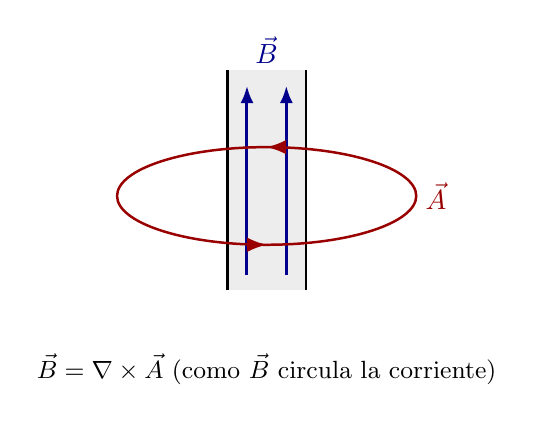
\begin{tikzpicture}[line width=0.9pt,>={Latex[length=2.2mm]}]
  % tubo de flujo B (vertical)
  \fill[black!7] (-0.5,-1.4) rectangle (0.5,1.4);
  \draw (-0.5,-1.4)--(-0.5,1.4) (0.5,-1.4)--(0.5,1.4);
  \foreach \x in {-0.25,0.25} \draw[->,blue!55!black,line width=1.1pt] (\x,-1.2)--(\x,1.2);
  \node[blue!55!black] at (0,1.65){$\vec B$};
  % A circulando alrededor (elipse horizontal)
  \draw[red!60!black,decoration={markings,mark=at position 0.25 with {\arrow{Latex}},mark=at position 0.75 with {\arrow{Latex}}},postaction={decorate}] (0,-0.2) ellipse (1.9 and 0.62);
  \node[red!60!black] at (2.15,-0.2){$\vec A$};
  \node at (0,-2.4){\small $\vec B=\nabla\times\vec A$ (como $\vec B$ circula la corriente)};
\end{tikzpicture}
\end{document}
